\subsection{Motivations}

\begin{frame}{Briefly review the learners' activities during RKB}

\begin{figure}[tb]
    \begin{center}
        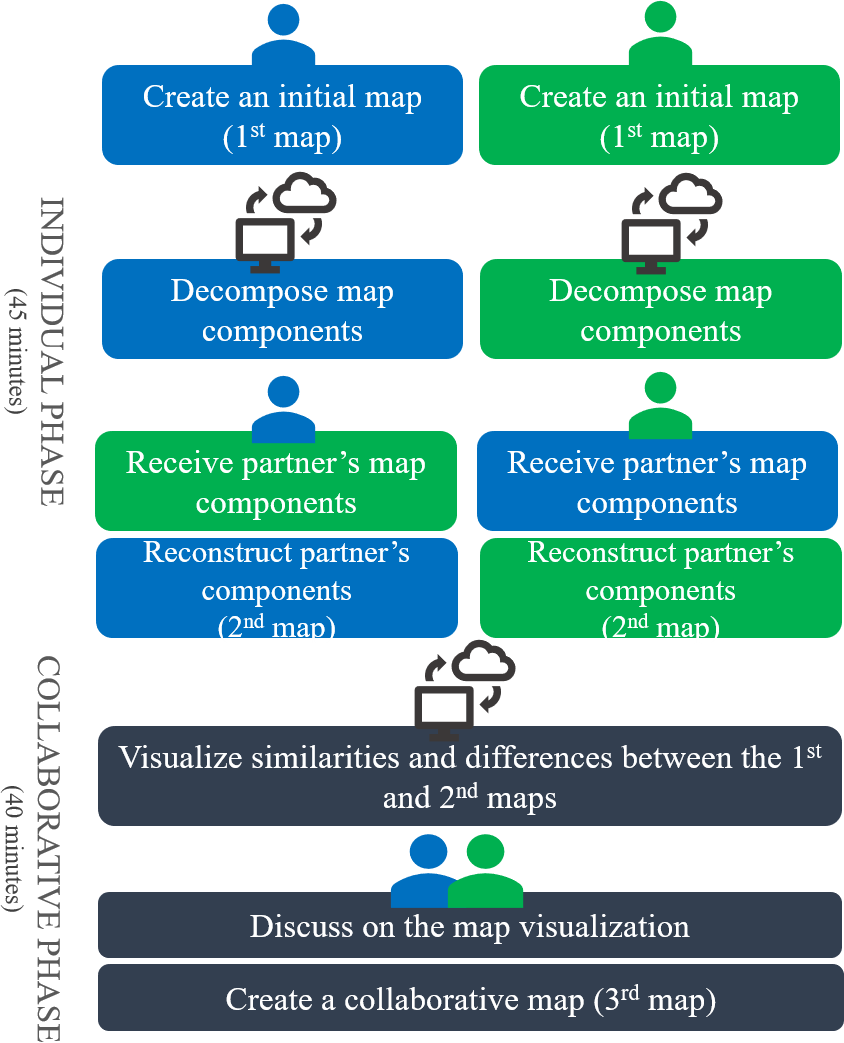
\includegraphics[width=55mm]{images/rqb_learner-activities.pdf}
    \end{center}
%    \caption{}
%    \label{prior_comprehension_dist}
\end{figure}
       
\end{frame}

\begin{frame}{Background}

\begin{itemize}
    \item A preliminary study on RKB for collaborative learning has explained \textcolor{blue}{how the approach affects collaborative learning outcomes and students’ learning experiences \cite{Sadita2018PreliminaryLearning}}; however, it does not investigate how similarity of prior knowledge convergence and comprehension of partner's representation (\textcolor{blue}{during individual phase}) may potentially influence the final collaborative product.
    \item Identifying the relationship between the individual and group product is important since there is interdependence between these two. 
\end{itemize}
       
\end{frame}

\begin{frame}{Research objectives}

\textcolor<1>{blue}{Aim}: To investigate how individual prior knowledge convergence and comprehension levels through reconstruction may potentially predict the final collaborative product

\begin{block}{Sub-research questions}
    \begin{enumerate}
        %\setcounter{enumii}{1}
        \item <+-> Does similarity of individual prior knowledge and/or comprehension 
              of partner's representation \textcolor{blue}{predict group learning outcomes}?
        \item <+-> How similarity of individual prior knowledge and comprehension
              of partner's representation \textcolor{blue}{contribute to} group learning outcomes?
    \end{enumerate}
\end{block}

\begin{itemize}
    \item <+->{\small The results of this study highlight the role of individual phases of RKB activities in \textcolor{teal}{foreseeing students’ learning achievements} as a group.}
s
\end{itemize}
    
\end{frame}



\subsection{Analysis methods}
\begin{frame}{Measurements for data analysis}
    \begin{itemize}
        \item <1-> Similarity of prior knowledge based on ind. \textcolor{blue}{initial maps}
        \item <1-> Comprehension of partner's understanding based on the ind. \textcolor{blue}{KB maps}
        \item <2> Map score changes based on the \textcolor{blue}{expert's evaluation} of students' initial and group maps
    \end{itemize}
\end{frame}

\begin{frame}{1) Similarity of prior knowledge: formulae}
    \begin{itemize}
        \item A graph \textit{G} = (\textit{V}, \textit{E}) is a finite set $V$ 
        of $n$ nodes and a set \textit{E} of edges, where \textit{E} is a 
        subset of $V \times V$.
        \item Given two undirected and labeled graphs, $A = (V, E_A)$ and 
        $B = (V, E_B)$, with common node set $V$, $S(A, B)$ is the similarity 
        between $A$ and $B$ as measured by $S$. 
        \item $SE_{AB}$ consists of shared links between $E_A$ and $E_B$ 
        while $UE_{AB}$ contains a set of unshared links created by 
        only one of the group members.
    \end{itemize}
\end{frame}

\begin{frame}{1) Similarity of prior knowledge: formulae (cont'd)}
    \begin{equation}
      SE_{AB} = E_A \cap E_B \label{eq:1}
    \end{equation}
    
    \begin{equation}
      UE_{AB} = E_A \ominus E_B \label{eq:2}
    \end{equation}
    
    \begin{equation}
      S(A, B) = \frac{|SE_{AB}|}{{|SE_{AB}| + \frac{|UE_{AB}|}{2}}} \label{eq:3}
    \end{equation}
    
    $S(A, B)$ represents \textcolor{blue}{the similarity score of two initial maps}
\end{frame}

\begin{frame}{1) Similarity of prior knowledge: linking words similarity}
    \begin{itemize}
        \item Pre-processing techniques: text normalization 
              (e.g., transforming to lower case, removing punctuation, stemming) 
              and stop-word removal
        \item Applying \textcolor{blue}{Term Frequency - Inverse Document Frequency (TF-IDF) cosine similarity} formula to get the linking-word similarity
        \item It falls into three following categories: 
        \begin{itemize}
            \item \textbf{no similarity} if the score is 0; 
            \item \textbf{moderately low similarity} if the score lies between 0--.509;
            \item \textbf{moderately high similarity} if greater than .509.
        \end{itemize} 
        \item This categorization is based on the first and third quartiles 
        of the similarity score distribution ($M = .27, SD = .34, Q1 = 0, Q3 = .509$).
    \end{itemize}
\end{frame}

\begin{frame}{2): Comprehension of partner's map components}

\begin{itemize}
    \item <+-> A graph $G_A = (V, E_A)$ is a finite set $V$ of $n$ nodes and a set $E$ of edges built by student $A$. 
    \item <+-> A graph $R_A = (V, E_{RA})$ is a graph re-constructed by student $A$'s partner. 
    \item <+-> Let $E_{MA}$ be the set of $A$'s first map links that are connected to the same nodes by the partner in the second map, while $E_{NA}$ consists of the links that are joined to different nodes.
    \item <+-> \begin{equation}
            E_{MA} = E_{RA} \cap E_A 
    \end{equation}
    \item <+-> \begin{equation}
            E_{NA} = E_{RA} \ominus E_A
    \end{equation}
    \\
    \item <+-> The element of $E_{MA}$ is called a reconstructed link, while $E_{NA}$ consists of non-reconstructed links.
\end{itemize}

\end{frame}

\begin{frame}{2): Comprehension of partner's map components (cont'd)}

Given two undirected and labeled re-constructional graphs $R_A$ and $R_B$ with common node set $V$, 
$C(A, B)$ is the comprehension value between student $A$ and $B$, as a pair in a group, defined as: 

\begin{equation}
  C(A, B) = \frac{|E_{MA} + E_{MB}|}{|E_{MA} + E_{MB}| + \frac{|E_{NA} + E_{NB}|}{2}} 
  \label{eq:6}
\end{equation}

\end{frame}

\begin{frame}{3)Similarity of individual and group map linking words}

\begin{itemize}
    \item Applying some pre-processing techniques and \textcolor{blue}{Term Frequency - Inverse Document Frequency (TF-IDF) cosine similarity} formula to get the linking-word similarity
    \item It falls into three following categories: 
    {\small \begin{itemize}
        \item \textbf{follow initial}: the group of linking words that are similar with at least one of the individual linking words (similarity value of equal to or more than .99);
        \item \textbf{modify initial}: the group of linking words that are modified from one of the individual linking words (similarity value above .366 and below .99);
        \item \textbf{new}: the group of linking words that are not similar to any of the individual linking words (similarity value of below .366).
    \end{itemize}} 
    \item This categorization is based on the first and third quartiles 
    of the similarity score distribution ($M = .68, SD = .37, Q1 = .366, Q3 = 1$).
\end{itemize}

\end{frame}

\begin{frame}{Data measurements (4): Map score change}

To measure the change of map score from the individual to the collaborative phase, this 
study adopts the normalized change formula proposed by Marx and Cummings 

%\cite{Marx2007NormalizedChange}.

\begin{equation}
 c =
    \begin{cases}
        \frac{gms - ais}{100 - ais} & \text{if $gms$ > $ais$}\\
        $drop$ & \text{if $gms$ = $ais$ = 100 or 0} \\
        0 & \text{if $gms$ = $ais$}\\
        \frac{gms - ais}{ais} & \text{if $gms$ < $ais$}
    \end{cases}
    \label{eq:7}
\end{equation}
    
\end{frame}


\subsection{Results \& discussions}
\begin{frame}{Results (1): Relationship Between Group Prior Knowledge Similarity, 
   Comprehension of the Partner’s Kit, and Map Score Change}

\begin{table}[tb]
    \caption{Descriptive statistics}
    \label{desc_stat}
    \begin{center}
        \begin{tabular}{c|c|c|c|c}
            \hline
            Data & $M$ & $SD$ & $Min$ & $Max$\\
            \hline
            $S(A, B)$ & .47 & .27 & 0 & .93 \\
            $C(A, B)$ & .85 & .12 & .65 & 1 \\
            & & & &\\
            $ais$ & 72.21 & 18.22 & 41.43 & 98.57 \\
            $gms$ & 90 & 7.31 & 75.71 & 100 \\
            $c$ & .54 & .34 & -.09 & 1 \\
            \hline
        \end{tabular}
    \end{center}
\end{table}
\end{frame}


\begin{frame}{Results (1): Relationship Between Group Prior Knowledge Similarity, 
   Comprehension of the Partner’s Kit, and Map Score Change}
    \begin{columns}
        \begin{column}{0.5\textwidth}
            \begin{center}
                \begin{figure}[tb]
                    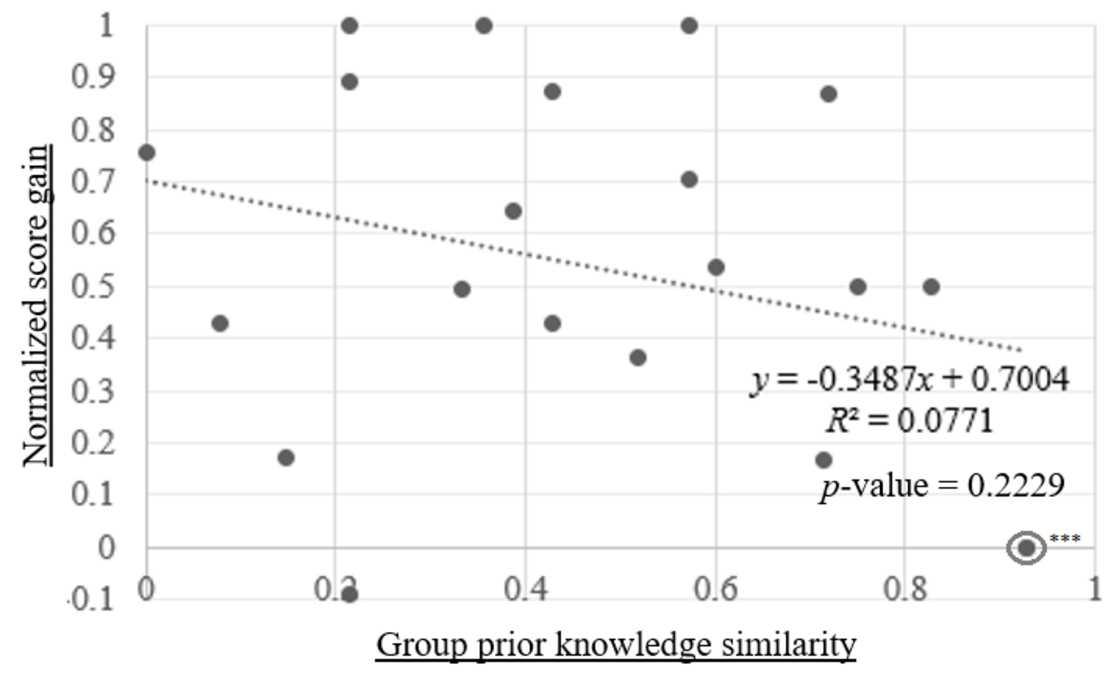
\includegraphics[width=50mm]{/images/a3_prior_gain_plot.pdf}
                    %\caption{Scatter plot of group prior knowledge similarity and normalized gain from individual to collaborative map}
                    \label{prior_gain}
                \end{figure}
            \end{center}
        \end{column}
        \begin{column}{0.5\textwidth}  %%<--- here
            \begin{center}
                \begin{figure}[tb]
                    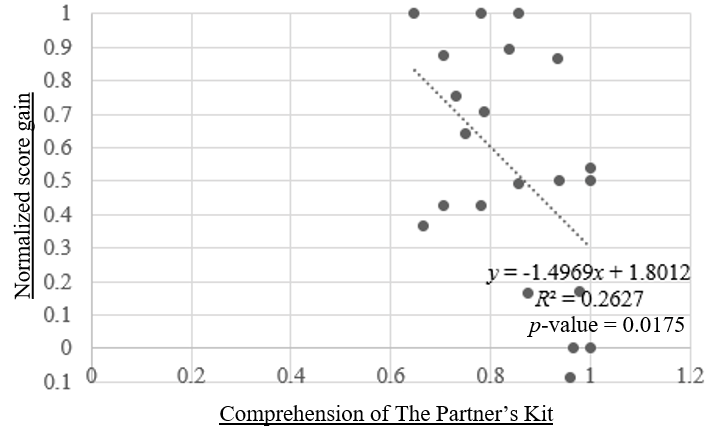
\includegraphics[width=50mm]{/images/a3_comprehension_gain_plot.pdf}
                    %\caption{Scatter plot of group comprehension level and normalized gain from 
                    %individual to collaborative map}
                    \label{comprehension_gain}
                \end{figure}
            \end{center}
        \end{column}
    \end{columns} 
\end{frame}


\begin{frame}{Result (1)}

\begin{itemize}
    
    \item <1-2> {\small Pearson’s correlation analysis shows that comprehension level and normalized change of products from individual to group level shows a \textcolor{teal}{moderately negative correlation}, with a significant coefficient, while similarity of prior knowledge reveals a \textcolor{purple}{weaker correlation with normalized change}.} 
    \item <2> {\small The \textcolor{teal}{comprehension of the partner’s representation is a stronger predictor} to detect the normalized change when compared to the similarity of prior knowledge.}
    \item <3-4> {\small A Wilcoxon signed-rank test indicates that the median of \textcolor{teal}{the similarity score between students' second maps and their partners' first maps $(Mdn = .746)$ is significantly higher} than the median of the similarity score between students' second and first maps $(Mdn=.6), Z= 224.5, p<0.01$.}
    \item <4> {\small Providing the partner's map components prompted students to reflect their understanding of their partner's representation.}

\end{itemize}

\end{frame}

\begin{frame}{Results (1): Similarity map distribution from the initial pair link and re-constructional map link}
\begin{figure}[tb]
    \begin{center}
        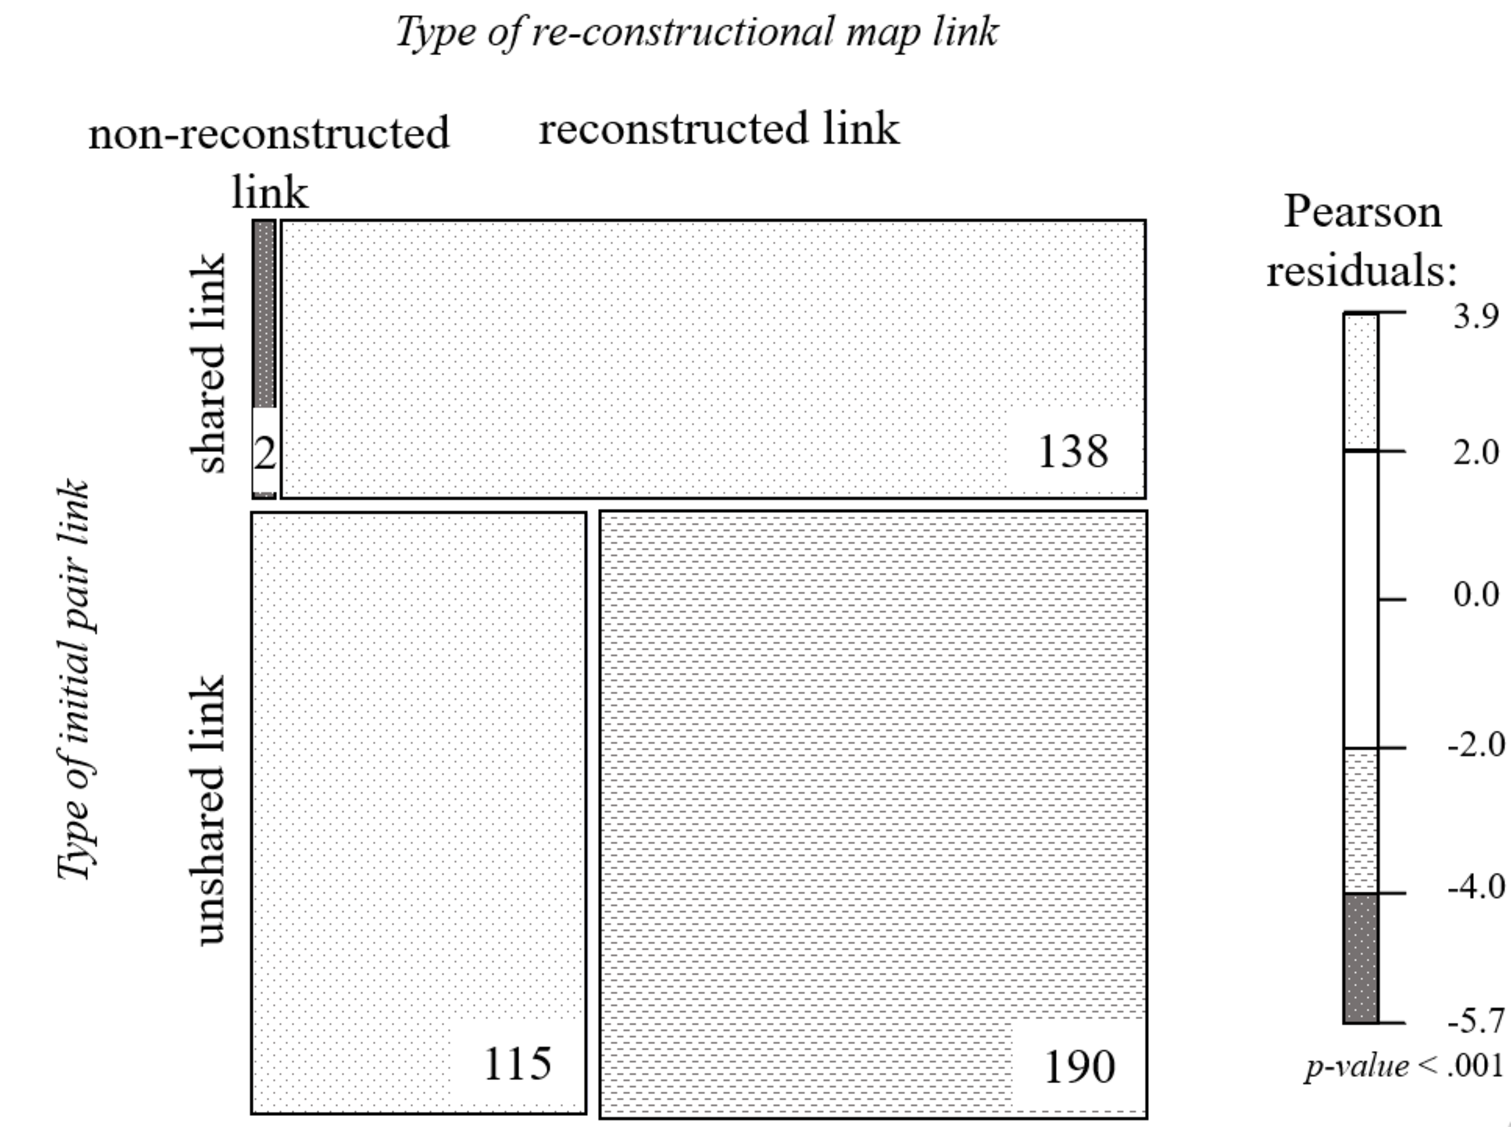
\includegraphics[width=60mm]{images/a3_prior_comprehension_distribution.pdf}
    \end{center}
    \caption{Almost all shared links can be reconstructed (99\%, \textit{n} = 138). The number of unshared links which can be reconstructed is higher than that for non-reconstructed links (\textit{n} = 115)}
    \label{prior_comprehension_dist}
\end{figure}
\end{frame}

\begin{frame}{Results (2): Individual Contributions to Collaborative Products}
    \begin{figure}[tb]
        \begin{center}
            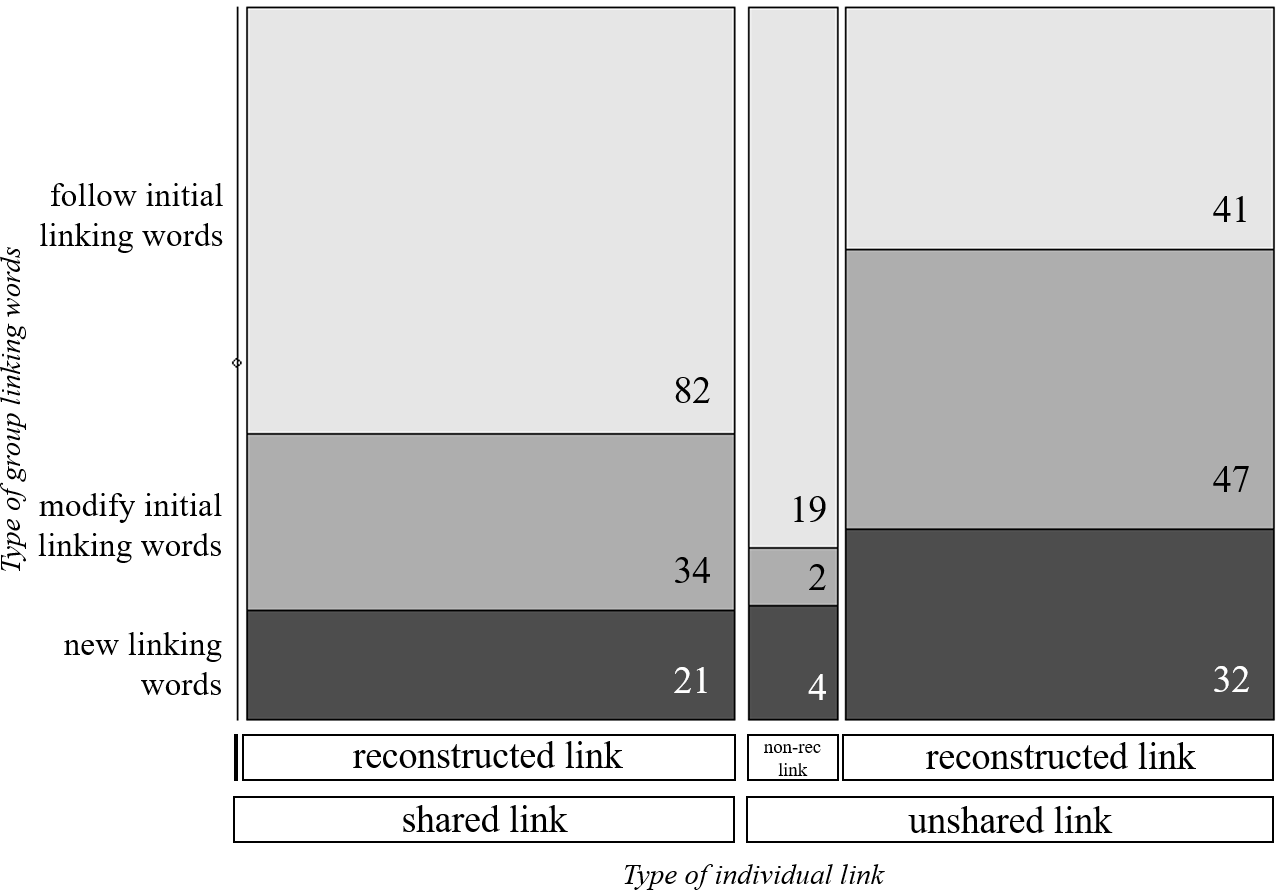
\includegraphics[width=60mm]{/images/a3_group_link_source_1.pdf}
        \end{center}
        \caption{Distribution of shared, unshared, reconstructed, and non-reconstructed links across all group maps. Both shared and unshared links contributed proportionally to the group map ($n$ = 137 and $n$ = 145, respectively). The reconstructed shared and unshared links were more likely to be accepted than the group links.}
        \label{group_link_s1}
    \end{figure}
\end{frame}



\begin{frame}{Results (2): Transfer of individual linking words to group map}
    \begin{figure}[tb]
        \begin{center}
            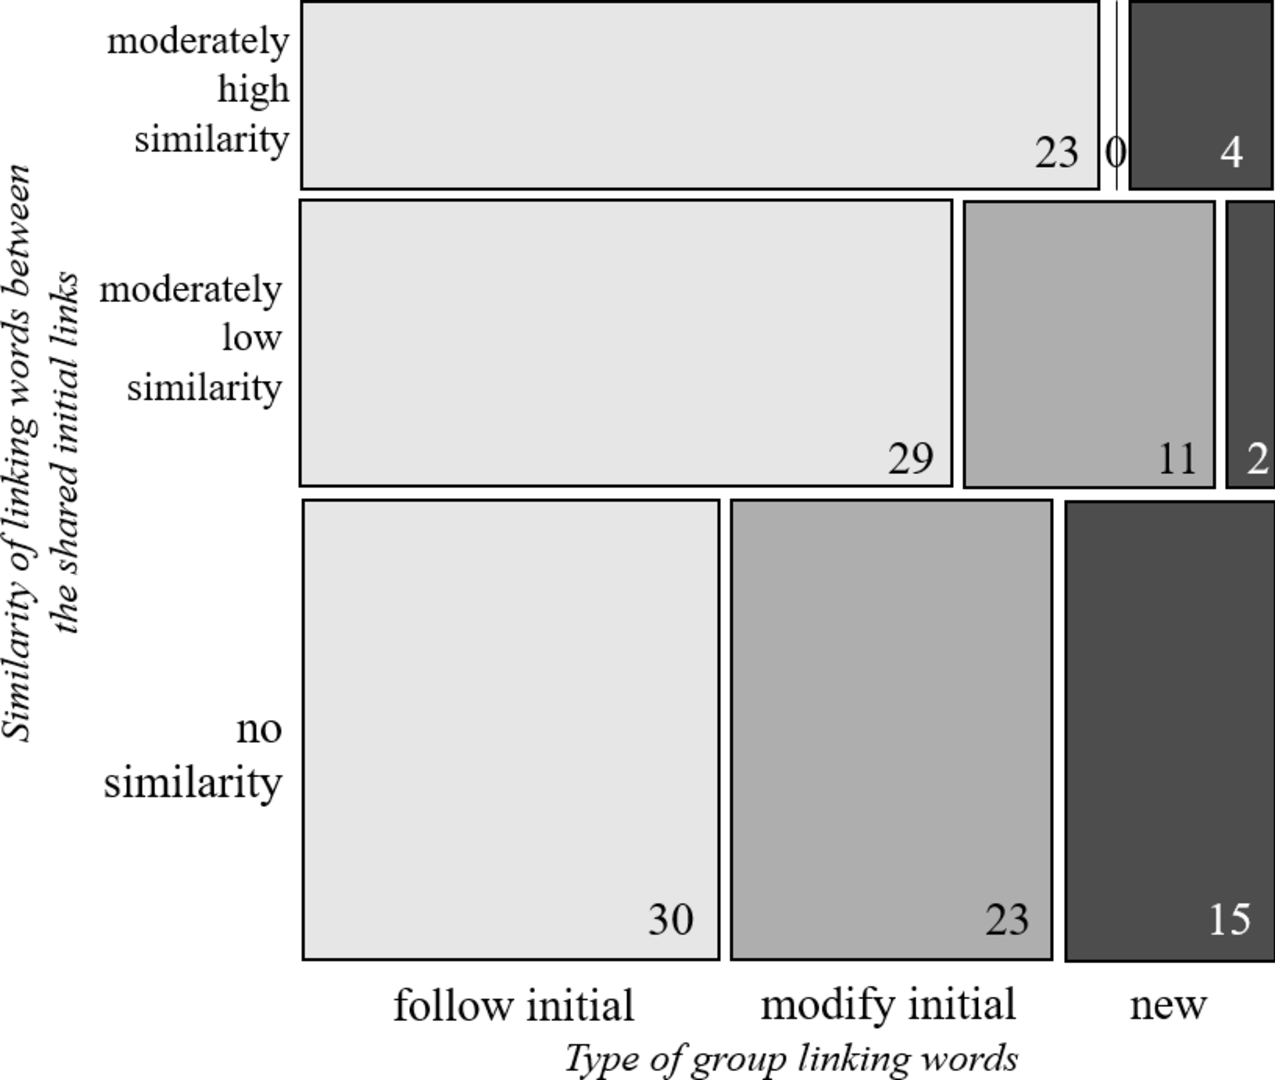
\includegraphics[width=45mm]{/images/a3_group_link_source_2.pdf}
        \end{center}
        \caption{{\footnotesize When the similarity of initial linking words is \textcolor{blue}{moderately high}, the tendency is to \textcolor{teal}{use any group member's initial} linking words without modifications. In cases when the similarity is moderately \textcolor{blue}{low}, \textcolor{teal}{any of the group member's linking words could be chosen} (69\%, $n$ = 29). However, the tendency is to \textcolor{teal}{modify or create new linking words} (56\%, $n$ = 38) when there is \textcolor{blue}{no similarity}.}}
        \label{group_link_s2}
    \end{figure}
\end{frame}


\begin{frame}{Summary of findings}
\begin{block}
    
\begin{itemize}
    \item <1> The results show that the \textcolor{teal}{comprehension of the partner's representation is a stronger predictor} to detect the normalized change when compared to the similarity of prior knowledge.
    \item <2> When students reconstructed their partners' components, they were making an effort to \textcolor{teal}{understand their partners' maps}, rather than to express their own initial maps by using new components. 
    \item <3-> There is an indication that the students were \textcolor{teal}{reflecting on their individual available knowledge} to construct the group product. 
    \item <4> \textcolor{teal}{Reconstruction trigger reflection and exploration activity}, enabling group members to review each other's representation.
\end{itemize}

\end{block}
\end{frame}




